\begin{frame}{GNU Make}
  \begin{center}
    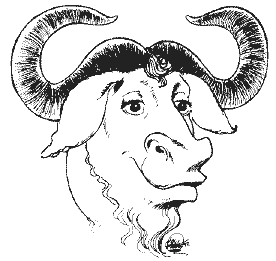
\includegraphics[scale=0.5]{logos/gnu.png}
  \end{center}
\end{frame}

\begin{frame}{Automatisierte, reproduzierbare Prozesse}
  Problem:
  \begin{itemize}
    \item kurz vor Abgabe noch die neuesten Korrekturen pullen
      \begin{itemize}
        \item Tippfehler korrigiert, Plot bearbeitet
      \end{itemize}
    \item \TeX{} ausführen, ausdrucken
    \item vergessen, Plot auszuführen
  \end{itemize}
  Lösung: Make!
  \begin{itemize}
    \item sieht, welche Dateien geändert wurden
    \item berechnet nötige Operationen
    \item führt Python-Skript aus, führt \TeX{} aus
  \end{itemize}
\end{frame}

\begin{frame}{Makefile}
  \begin{itemize}
    \item Datei heißt \texttt{Makefile}, keine Endung!
    \item besteht aus Rules:
  \end{itemize}
  \begin{block}{Rule}
    \texttt{target: prerequisites\\
    \hspace{1cm} recipe}
  \end{block}
  \begin{description}
    \item[\texttt{target}] Datei (oder mehrere), die von dieser Rule erzeugt wird
    \item[\texttt{prerequisites}] Dateien, von denen diese Rule abhängt
    \item[\texttt{recipe}] Befehle, um \texttt{target} aus \texttt{prerequisites} zu erstellen
  \end{description}
\end{frame}

\begin{frame}{Beispiel}
  \texttt{all: report.pdf\\[0.5cm]
    plot.pdf: plot.py daten.txt\\
    \hspace{1cm} python2 plot.py\\[0.5cm]
    report.pdf: report.tex plot.pdf\\
    \hspace{1cm} latex report.tex\\[0.5cm]
    .PHONY: all
  }

  \begin{itemize}
    \item wenn nur \texttt{make} gestartet wird, wird der erste Target erstellt, hier \texttt{all}
    \item \texttt{all} braucht \texttt{report.pdf}, also wird er erzeugt
    \item \texttt{report.pdf} braucht noch \texttt{plot.pdf}, also wird Python ausgeführt
    \item Die letzte Zeile bewirkt, dass \texttt{make} weiß, dass \texttt{all} keine echte Datei ist
  \end{itemize}
\end{frame}
